
\chapter{Expressionism and Serialism}
\label{twentieth}

Although serialism here is mentioned it really only appears rigorously in the Webern. 
Prior to this we see two pieces by Webern's colleagues, Schoenberg and Berg.
Both use the voice; both are highly expressionistic in nature. 


\section{Schoenberg: Pierrot Lunaire}
\begin{itemize}
\item Listen: \url{https://www.youtube.com/watch?v=N-zW10__i4M}
\item Score: \url{http://imslp.org/wiki/Pierrot_Lunaire,_Op.21_%28Schoenberg,_Arnold%29}
\item Reading: \url{http://www.jstor.org/stable/pdfplus/10.2307/832890.pdf}
\end{itemize}

Expressionism began in paint such as Franz Marc, Emil Nolde and Vasily Kandinsky. Marc and Kandinsky are associated with the \textit{Blaue Reiter} movement; Nolde is better associated with Die Br\"uke - the Bridge, a similar group of expressionist artists. Primitive arts and expressive use of colour triggered an emotional search for the spiritual. Kandinsky's \textit{Der Blaue Reiter} of 1903 gave the group its name. Schoenberg was a member of this group being as he was both an accomplished musician and painter. Although \textit{Der Blaue Reiter} sought the spiritual, it moved towards the abstract (note a gradual move towards cubist tendencies), the subjective (introspective) and the avant-garde. 

Thus, Schoenberg's early works develop the idea of `going beyond'. 

\textit{Verkl\"arte Nacht (Transfigured Night)} from 1899 is inspired by a poem by Richard Dehmel of the same name. 

\begin{table}[h!]
\begin{tabular}{|l|l|} \hline
Zwei Menschen gehn durch kahlen, kalten Hain; & Two people are walking through a bare, cold wood;\\
der Mond l\"auft mit, sie schaun hinein. & the moon keeps pace with them and draws their gaze.\\
Der Mond l\"auft über hohe Eichen; & The moon moves along above tall oak trees,\\
kein W\"olkchen tr\"ubt das Himmelslicht, & there is no wisp of cloud to obscure the radiance\\
in das die schwarzen Zacken reichen. & to which the black, jagged tips reach up.\\
Die Stimme eines Weibes spricht: & A woman’s voice speaks:\\	  	
\hline
``Ich trag ein Kind, und nit von Dir, & ``I am carrying a child, and not by you.\\
ich geh in S\"unde neben Dir. & I am walking here with you in a state of sin.\\
Ich hab mich schwer an mir vergangen. & I have offended grievously against myself.\\
Ich glaubte nicht mehr an ein Gl\"uck & I despaired of happiness,\\
\hline
und hatte doch ein schwer Verlangen & and yet I still felt a grievous longing\\
nach Lebensinhalt, nach Muttergl\"uck & for life’s fullness, for a mother’s joys	\\
\hline
und Pflicht; da hab ich mich erfrecht, & and duties; and so I sinned,\\
da lie{\ss} ich schaudernd mein Geschlecht & and so I yielded, shuddering, my sex\\
von einem fremden Mann umfangen, & to the embrace of a stranger,\\
und hab mich noch daf\"ur gesegnet. & and even thought myself blessed.\\
Nun hat das Leben sich ger\"acht: & Now life  has taken its revenge,\\
nun bin ich Dir, o Dir, begegnet.'' & and I have met you, met you.'' \\	
\hline
Sie geht mit ungelenkem Schritt. & She walks on, stumbling.\\
Sie schaut empor; der Mond l\"auft mit. &  She looks up; the moon keeps pace.\\
Ihr dunkler Blick ertrinkt in Licht. & Her dark gaze drowns in light.\\
Die Stimme eines Mannes spricht: & A man’s voice speaks:\\
\hline
``Das Kind, das Du empfangen hast, & ``Do not let the child you have conceived\\
sei Deiner Seele keine Last, & be a burden on your soul.\\
o sieh, wie klar das Weltall schimmert!  & Look, how brightly the universe shines!\\
Es ist ein Glanz um alles her; & Splendour falls on everything around,\\
Du treibst mit mir auf kaltem Meer, & you are voyaging with me on a cold sea,\\
doch eine eigne W\"arme flimmert & but there is the glow of an inner warmth\\
von Dir in mich, von mir in Dich. & from you in me, from me in you.\\
Die wird das fremde Kind verkl\"ren, & That warmth will transfigure the stranger’s child,\\
Du wirst es mir, von mir geb\"ren; & and you bear it me, begot by me\\
Du hast den Glanz in mich gebracht, & You have transfused me with splendour,\\
Du hast mich selbst zum Kind gemacht''. & you have made a child of me.''\\
\hline
Er fa{\ss}t sie um die starken H\"uften. & He puts an arm about her strong hips.\\
Ihr Atem k\"u{\ss}t sich in den L\"uften. & Their breath embraces in the air.\\
Zwei Menschen gehn durch hohe, helle Nacht. & Two people walk on through the high, bright night.\\
\hline
\end{tabular}
\caption{Verkl\"arte Nacht (Transfigured Night), Richard Dehmel}
\label{tab:faune}
\end{table}

It is scored for string sextet although there is a version for string orchestra. Its harmonies are clear but there is an increased chromatic contrapuntalism, inherited from Wagner and also heard in Mahler and Strauss. 
The poem is highly charged and this desire is reflected in the music through wrought melodies and rising sequences. 

A \textit{Pelleas und Melisande} followed in 1899. The Maeterlinck play (1893) was hugely popular at the time and its theme of love, jealousy and death played completely into the expressionist's hand. The music has grief-stricken passion with huge chords and vast changes of orchestral density. Schoenberg's \textit{Chamber Symphony no.1} pushed the boundaries of harmony even further and coincided with the writing of his treatise on harmony in 1910 (published in 1922). 

The \textit{Five Orchestral Pieces} Op.9 of 1909 is notable for the development of \textit{Klangfarbenmelodie}. Only through orchestration does the music develop: there is hardly any melodic or rhythmic articulation. 

This pushing at the boundaries was noticed even by Schoenberg himself. Of his song-cycle \textit{Das Buch der hangenden Garten} Op.15 from 1910 he wrote, I have `broken through every restriction of a bygone aesthetic'. He explained that he had emancipated dissonance - that a chord could resolve this way and that and be equally acceptable. Debussy had done something similar with his non-functional harmony. 

\begin{figure}[H]
\centering
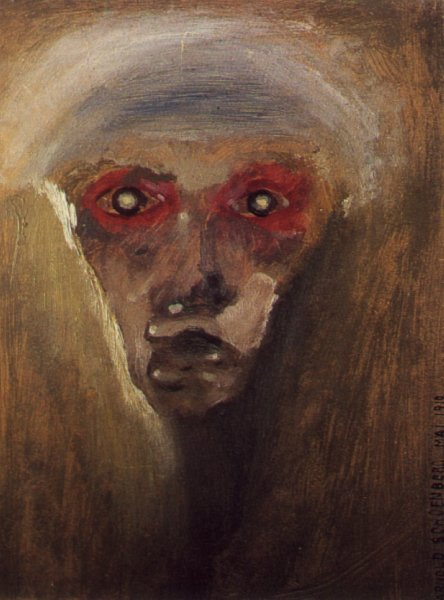
\includegraphics[scale=0.8]{roteblick}\caption{Der Rote Blick - the Red Gaze (1910)}
\label{fig:roteblick}
\end{figure}

Two music dramas followed in quick succession: \textit{Ewartung} (expectation) for soprano and orchestra (1909) and \textit{Die gl\"uckliche Hand} (the lucky hand) for voices and orchestra (1910/13). In \textit{Ewartung} we hear the hidden thoughts of a woman waiting in the forest for her lover (a Pelleas version again). The synopsis is as follows:

\begin{quotation} 
A woman is in an apprehensive state as she searches for her lover. In the darkness, she comes across what she first thinks is a body, but then realises is a tree-trunk. She is frightened and becomes more anxious as she cannot find the man she is looking for. She then finds a dead body, and sees that it is her lover. She calls out for assistance, but there is no response. She tries to revive him, and addresses him as if he were still alive, angrily charging him with being unfaithful to her. She then asks herself what she is to do with her life, as her lover is now dead. Finally, she wanders off alone into the night.
\end{quotation}

The madness of the tortured mind develops further still with \textit{Pierrot Lunaire} of 1912 for voice and small ensemble comprising piano, flute (pic), clarinet (bass), violin (viola) and cello. Whilst many note this piece as pivotal for its use of Sprechstimme (a kind of semi-pitched vocalisation) this piece projects Schoenberg's own fascination with (and suspiciousness of) numbers. 

Who was Pierrot? Pierrot was a pantomime character and is commonly represented as a sad clown. Columbine is the object of his desires; Harlequin the object of hers. Thus again a love triangle with Pierrot originally the object of ridicule but during Symbolist times, the ultra-sensitive loner with only the moon for company.  

The structure of the work is as three times seven poems drawn from Albert Giraud's writings from 1884 (original in French with German translation by Otto Hartleben).  

\begin{table}[h!]
\begin{tabular}{|p{5.0cm}|p{5.0cm}|p{5.0cm}|} \hline
\textbf{Part One} & \textbf{Part Two} & \textbf{Part Three} \\\hline
Mondestrunken (Moondrunk) & Nacht (Passacaglia) (Night) & Heimweh (Homesickness)\\\hline
Columbine & Gebet an Pierrot (Prayer to Pierrot) & Gemeinheit! (Vulgarity)\\\hline
Der Dandy (The Dandy) & Raub (Theft)  & Parodie (Parody)\\\hline
Eine blasse W\"ascherin (An Ethereal Washerwoman) &  Rote Messe (Red Mass) & Der Mondfleck (The Moonspot)\\\hline
Valse de Chopin (Chopin Waltz) & Galgenlied (Gallows Song)  & Serenade\\\hline
Madonna & Enthauptung (Beheading) & Heimfahrt (Barcarole) (Homeward Bound)\\\hline
Der kranke Mond (The Sick Moon) & Die Kreuze (The Crosses) & O Alter Duft (O Ancient Fragrance)\\\hline
\end{tabular}
\caption{Pierrot Lunaire, 1912}
\label{tab:pierrot}
\end{table}

The stark rendition (especially when semi-staged) and the numerological references are well worth further investigation. 

As Schoenberg paired down the notational script of music so to did his works become more conceptual in size. 
His most famous students were Anton Webern and Alban Berg. Although Berg would follow his composition teacher down the serial road, he was always concerned with larger forms which serialism would not sustain. Webern however was not worried about this and as a consequence his complete oeuvre can be found on just three compact discs. 

Schoenberg's later works including the \textit{Variations for orchestra} (1926/28), \textit{Violin concerto} (1934/36), \textit{String quartet No. 4} (1936), \textit{Piano concerto} (1942), \textit{String Trio} (1946)
and the six minute \textit{A Survivor from Warsaw} (1947) are well worth following up. 
 
\section{Berg: Wozzeck}
\begin{itemize}
\item Listen: \url{https://www.youtube.com/watch?v=uUkbjO8dkDI}
\item Reading: \url{http://adrian-moore.staff.shef.ac.uk/teaching/mus126/wozzeck.pdf}
\end{itemize}

Amongst numerous song cycles, key works of Alban Berg (1885-1935) to follow up are:
\begin{itemize}
\item Piano Sonata Op.1 (1907)
\item String quartet Op.3 (1910)
\item Wozzeck Op.7 (1914-22)
\item Lyric Suite (string quartet, 1925-6)
\item Lulu (1929-35)
\item Violin concerto (1935) 
\end{itemize}

Berg's early life was not a happy one. At age 18, his father had died, the family was poor, Alban's health was unsteady, he was not successful intellectually, he was unhappy in love yet had fathered an unwanted child. Berg attempted suicide. 

Berg's early career was heading towards accountancy when he met Schoenberg. He learned his trades quickly and although poor, was gifted an inheritance in 1905 which allowed him to resign his government job in 1906. In Schoenberg's class Berg quickly became friends with Anton von Webern. Webern we know was killed in September 1945, in Mittersill, near Salzburg. He had stepped out of his son-in-law's house for a smoke and was shot by an American soldier. 

Musically Berg and Webern went separate ways: Berg looked to the past, Webern to an uncertain future. Though both men knew the risks they were taking. Egon Wellesz recounts the premiere performance of Schoenberg's Op.10 quartet: (\href{http://conquest.imslp.info/files/imglnks/usimg/c/c1/IMSLP29725-PMLP66179-Schoenberg_-_SQ_No._2_score.pdf}{score})

\begin{quotation}
The atmosphere in the elegant and old-fashioned Boesendorfer Hall was tense from the beginning ... The first movement had hardly begun when, enraged by the unexpected C in the fifth bar, the music critic named Karpath jumped up from his seat and shouted, ``Stop it!'' Unperturbed, the Rose Quartet went on; but it was in that scherzo that, after a \textit{fortissimo}, the audience started laughing and its laughter drowned out the music. An elderly gentleman sitting in front of Mahler began whistling on a door key. I heard Mahler shouting, ``I'll risk five florins (the fine for disturbing the peace) and box you on the ear!'' ``You are not here as director of the Opera, you can't order me to stop,'' the man retorted. Mahler rose from his seat, but at that moment two young men, pupils of Schoenberg, rushed forward and carried the man out of the hall.
\end{quotation}

We should be careful of Karen Monson's regurgitation of this vignette. The premiere of the second quartet was December 1908. Mahler was in the states at this time. 

By the summer of 1907 Berg had been studying harmony and counterpoint with Schoenberg for over two years and was ready to undertake original composition. After numerous small song cycles, Berg began his piano sonata: a planned three movements. Only one transpired and Schoenberg said that was enough. (\href{http://petrucci.mus.auth.gr/imglnks/usimg/7/75/IMSLP234327-SIBLEY1802.21900.4ff7-39087012041663score.pdf}{score})
For all its chromaticism this work is in sonata form and Bminor. 

We should remind ourselves that Berg and Webern were composing at a time of huge Bruckner symphonies were only 10 years old, Strauss was writing virtuoso tone poems and Mahler was conducting his own symphonies. 
Berg was friends with the artist Gustav Klimt and Klimt was the Damien Hurst of his age. 

Berg's first string quartet was premiered on April 24, 1911, just before his wedding to Helene Nahowski. At this point in his life he took his leave as student from Schoenberg. 

On May 3rd, 1911 he married Helene but finances were still tight. For work, Berg (who had been signed to Universal through solid success with the quartet) began copying parts and making piano reductions of scores (mainly Schoenberg's). Schoenberg was working on \textit{Gurrelieder}, the apogee of orchestral and choral forces - something requiring a new kind of score paper to be produced. It is interesting to note Berg's (and to an extend Webern's) slavish duty to their master.  

Berg began work on a large scale piece based upon poems by his friend Peter Altenberg. The premiere of the \textit{Five Altenberg Lieder} was March 31, 1913. The Vienna scandal was as riotous as the Parisian scandal for \textit{The Rite}. Berg's piece called for full forces but they were always used sparingly and there were huge contrasts in texture. Moreover, the pieces were remarkably short, the full cycle lasting just a little over 11 minutes. Not only did Berg feel hurt by the audience's reaction, the lieder then lapsed into the doldrums for many years. Berg managed to complete his Op.6, three orchestral pieces before war broke out. 

Schoenberg, Berg and Webern were patriotic (though Schoenberg was to suffer antisemitism from the early 20s) and and despite their best efforts were signed up but Berg was never going to be fit enough. New Year's Day, 1915, Berg wrote to Schoenberg `Life \textit{outside} goes on just as usual...As if nothing had happened, people in Vienna live completely without restraint, operettas and farces `adapted to the times' are produced, and every theater and cinema is filled to the bursting point.' Schoenberg, never of the best of health was released from the army in 1916 (by requests from Bart\'ok and many others). And as Italy got drawn into the war, Berg found himself being called up. His time in the army was, by all accounts, a torrid affair.  

\subsection{Wozzeck}
Berg drew the plot for \textit{Wozzeck} from the drama by Georg B\"uchner (1813-1837). B\"uchner was a radical: a communist before communism and an superior intellectual by all accounts - with training as a scientist. However it was writing that excited him. \textit{Woyzeck} was B\"uchner's third play. The play was drawn from history. In June 1821, in Leipzig, a 41 year old barber named Johann Christian Woyzeck stabbed his mistress, the widow Woost, in a fit of jealous rage. Despite being examined by doctors, evidence was given that Woyzeck was not of sound mind when he committed the crime (the first time diminished responsibility was used as a legal defence). Nevertheless, Woyzeck was beheaded. Woyzeck had told his doctor that he was having visions and had contemplated suicide in order to free himself. All in all Woyzeck represented the beleaguered and oppressed and became the symbol (a paraiah picked upon by society) for B\"uchner's play. Berg went to see the play in Vienna just before the war and decided there and then this would be the subject of his first opera.

And it is clear that whilst Berg had in mind the same orders of magnitude as a Wagner or Verdi opera, he did not know how to develop the form. Here we had a madman (Wozzeck) going up against the likes of Mimi, Tosca and Madame Butterfly. It takes a different kind of opera to make this work. Interesting to note the binding of scenes with short orchestral interludes. In letters to Webern, Berg ponders the issue of the vocal projection of \textit{Sprechstimme} in the opera theatre. Schoenberg was so impressed with the preliminary scores that he asked Universal to sign Berg's contract for the score so affording him more time to finish the work. Alas, even this was in vain. Berg really had to struggle to complete \textit{Wozzeck}. 

\begin{table}[h!]
\begin{tabular}{|l|l|} \hline
Scene & Music \\\hline
Act 1 - Wozzeck with others & Five character pieces \\\hline
1. Wozzeck and the Captain & Suite\\
2. Wozzeck and Andres & Rhapsody\\
3. Wozzeck and Marie & March and Lullaby\\
4. Wozzeck and the Doctor & Passacaglia\\
5. Marie and the Drum Major & Quasi Rondo\\\hline
Act 2 - Dramatic development: Symphony\\\hline
1. Marie, child, Wozzeck & Sonata movement\\
2. Captain, Doctor, Wozzeck & Fantasy and Fugue\\
3. Marie and Wozzeck & Largo\\
4. Garden of the Inn & Scherzo\\
5. Guard post, barracks & Rondo with introduction\\\hline
Act 3 - Catastrophe and epilogue: Six inventions\\\hline
1. Marie and child & Invention on a theme\\
2. Marie's death & Invention on a note\\
3. Tavern & Invention on a rhythm\\
4. Wozzeck's death & Invention on a chord of the 6th\\
Orchestral interlude & Invention on a Key (D minor) \\
5. Children playing & Invention in a perpetual motion\\\hline
\end{tabular}
\caption{Wozzeck, plan}
\label{tab:wozzeckplan}
\end{table}

Of all the technical feats in this opera the invention on a note is perhaps the best known. B-natural eschews itself into the scene, climaxing when Wozzeck stabs Marie. We hear it first in the depths (Double-bases) then as a shrill violin harmonic, then through glissanidi across the strings. It is \textit{ppp} across all strings when Marie sings `How the moon rises red!' Exit Wozzeck. Over the change of scene across six bars, we hear the crescendo from \textit{pppp} to \textit{fff}..twice for good measure. 

Look at the orchestration used (in particular the size of the orchestra versus the need to hear the singers). As a consequence we get a wash of expressionist colour. And the orchestra is divided even more rigorously by the use of H and N for Haupstimme (main voice) and Nebenstimme (next or secondary line). The score, is both heavily detailed and beautiful in design. No wonder as Berg had to copy the score himself, self-fund its promotion, surviving Schoenberg's criticism (some say that Schoenberg might have been a little jealous at his student's immanent success). Publication, though tortuous, was eventually secured through Universal. Berg met the conductor Hermann Scherchen, who suggested fragments of the opera be played in concert. This helped publicise the opera prior to its fully fledged premiere performance on 14th December 1925 under Erich Kleiber in Berlin. With a slightly cut back orchestration, Berg was able to obtain many more performances and by 1935 - the year of his death - \textit{Wozzeck} had been performed worldwide.  

\subsection{One or two important themes}

\begin{figure}[H]
\centering

\includegraphics[scale=0.2]{captain}\caption{The Captain}
\label{fig:captain}
\end{figure}


\begin{figure}[H]
\centering

\includegraphics[scale=0.2]{marie}\caption{Marie}
\label{fig:marie}
\end{figure}


\begin{figure}[H]
\centering

\includegraphics[scale=0.2]{death}\caption{Death}
\label{fig:death}
\end{figure}



\begin{figure}[H]
\centering
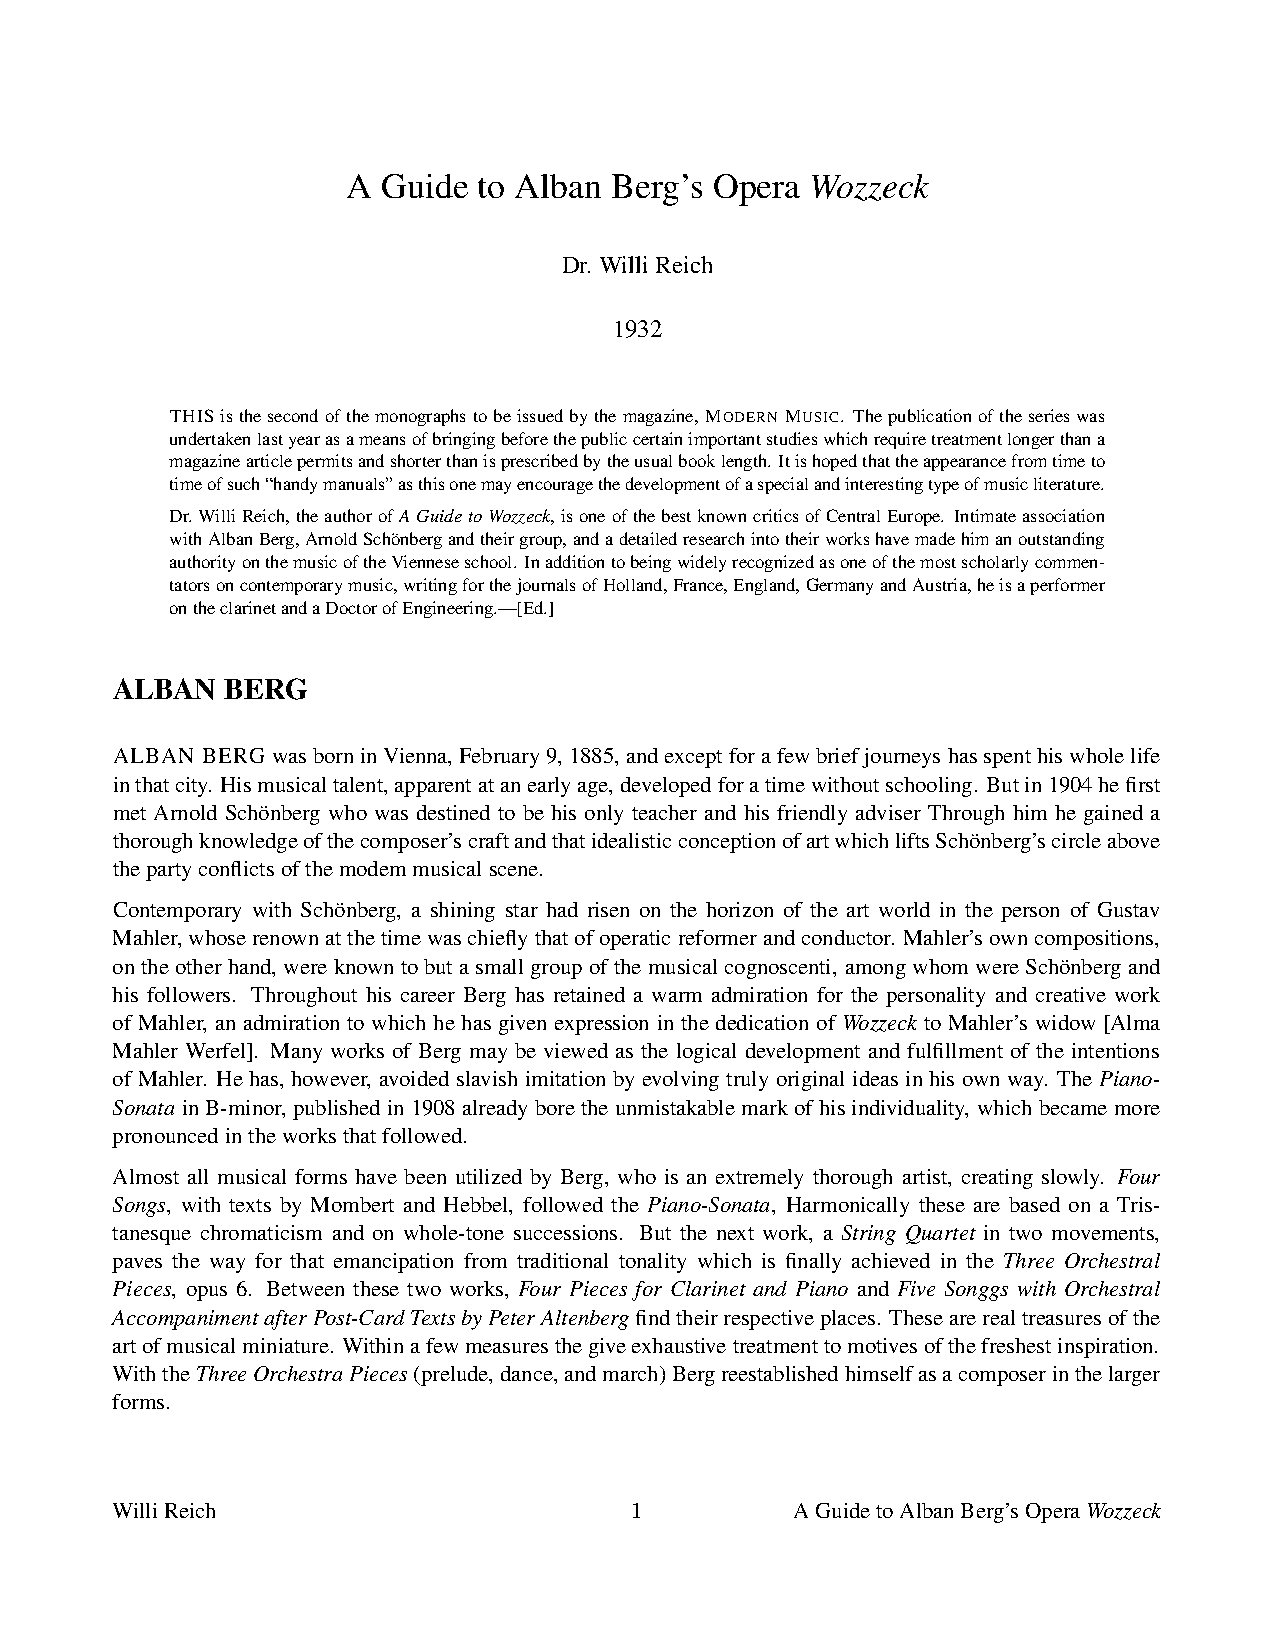
\includegraphics[scale=0.2]{wozzeck}\caption{Wozzeck}
\label{fig:wozzeck}
\end{figure}



\begin{figure}[H]
\centering

\includegraphics[scale=0.2]{knife}\caption{Knife}
\label{fig:knife}
\end{figure}

Important works after \textit{Wozzeck} include the Chamber concerto, the opera \textit{Lulu} (incomplete at the time of death), after plays by Frank Wedekind and the violin concerto.

The life of the Austrian-German composer in the 30s was terrible. The Nazi regime had basically stated that German music reached its pinnacle with Brahms. Schoenberg went to the United States in 1933, Webern allied himself with Nazis as he needed the work. 

\textit{Lulu} - a monumental work - was abandoned in 1935 as Berg accepted a commission to write the violin concerto. It too had a sad and distressful genesis. The composer died before the first performance (conducted by Webern) with the violinist Krasner (who had commissioned the work) in 1936, in Barcelona.  
 
%%%%%%%%%%%%%%%%%%%%%%%%%%%%%%%%%
\section{Webern: Concerto for nine instruments Op. 24}

\begin{itemize}
\item Listen: \url{https://www.youtube.com/watch?v=vmumBURcHlc}
\item Listen: \url{https://www.youtube.com/watch?v=rIr1xrunnf0}
\item Score: \url{http://imslp.org/wiki/Concerto,_Op.24_%28Webern,_Anton%29}
\end{itemize}

Early studies with Anton Komauer who introduced Webern to Wagner's music but also the songs of Hugo Wolf. Moreover, like Schoenberg, Komauer instilled a thorough grounding in harmony and counterpoint through intense study of Bach. Webern grew up with the music of Strauss and Mahler. Later in his studies, with Professor Guido Adler, Webern got to know the music of Josquin des Pr\`es, Johannes Ockeghem and Heinrich Isaac. Prior to his studies with Schoenberg, Webern had produced little of note, save perhaps for the orchestral work \textit{In Sommerwind}. 

Webern (1883-1945) enrolled in Schoenberg's classes - became friends with Berg - and in four years became a highly skilled composer. Webern was a gifted pianist and cellist and gradually he had to let these skills lapse in favour of composition. Webern's mother died in 1906, (Webern was 23) and this affected him greatly. Even his long-time love and soon to be wife, Wilhelmine M\"ortl realised where her place was in relation to Webern's mother. 

Webern persued a career as a conductor after finishing his graduate studies which wasn't easy. However he was adequately supported by his father and therefore continued his studies with Schoenberg. In 1908 Webern completed his opus 1, the \textit{Passacaglia} for orchestra. This work is grand in scale and intricate in harmonic detail. It comprises a short theme and 23 variations plus coda. 

\subsection{Webern Op.24}
 
\begin{figure}[H]
\centering

\includegraphics[scale=0.2]{webernop24row}\caption{Webern Op.24 Konzert: Row}
\label{fig:op24row}
\end{figure}

What is so important about this row is that each three note cell is a serial development from the first (RI, R, I).

\begin{figure}[H]
\centering

\includegraphics[scale=0.2]{webernrow4-1}\caption{Webern Op.24 Konzert: Row and expansion: Top row is O...what are the rest?}
\label{fig:op24row2}
\end{figure}

This row is given klangfarbenmelodie orchestration and intervallic expansion (minor 2nds becoming minor 9ths). It is clear that the rows are split between piano and the other instruments or shared between the two. The next entrance is piano:

\begin{figure}[H]
\centering

\includegraphics[scale=0.2]{webernop24row2-1}\caption{Webern Op.24 Konzert: Piano entry}
\label{fig:op24row}
\end{figure}



